As mentioned in the previous section the number of learning steps where a change was accepted. This could be because of a bad exploration of the coefficients in the partitions. The change we will make to the learning algorithm is as such: if a change made to the preconditioner did not improve the solver iteration count, we will try the same change on the same coefficient scaled by \(0.5\), if that worked the scaled change is accepted and continues as the original algorithm. If this scaled change also get rejected, the change will be scaled by \(0.25\). Then if all scaled changes does not improve the solver iteration count the algorithm continues as normal by generating a new change and a new coefficient is chosen. For pseudocode see Algorithm \ref{alg: leaning with scales}. Because the new version of the learning algorithm will test up to 3 times as many different preconditioners, therefore for the test to be comparable to the previous test we will use a base number of learning steps of 100 instead of 300. Other parameters of the algorithm will not be changed, table \ref{table: initial learn param}.

When comparing the result to the previous test the learned preconditioner is a small amount worse and the reason for the change to the algorithm also did not improve as the number of accepted preconditioners is also less, table \ref{table: initial change stat}. A positive improvement is that the learning curves are steeper meaning faster learning, figure \ref{fig: change of scale}. This is especially notable for the matrix fidap004 and might explained the fewer number of improvements. As now the algorithm finds the best preconditioner faster and can therefore find any more changes that would improve the preconditioner. Because the learned preconditioner are only a marginally worse and especially the faster learning, we will keep the change made to the learning algorithm.

\begin{algorithm}[H]
    \caption{Preconditioner learning algorithm with scaling of the change}\label{alg: leaning with scales}
    \begin{algorithmic}
        % \Require $n \geq 0$
        \Require Matrix \(A\) and vector \(b\) form \(Ax=b\)
        \State \(M^{-1} \gets \) Generate initial preconditioner
        \State \(k \gets\) Solver iteration count for \(M^{-1}Ax=M^{-1}b\)
        \Loop{ \( i=1,2,\ldots\)}
            \Loop { \(s=\left\lbrace 1, 0.5, 0.25\right\rbrace\)}
                \State \(M^{-1}_{new} \gets \) Changed \(M^{-1}\) with scale \(s\)
                \State \(k_{new} \gets\) Solver iteration count for \(M^{-1}_{new}Ax=M^{-1}_{new}b\)
                \If{ \(k_{new} < k\)}
                    \State \(k \gets k_{new}\)
                    \State \(M^{-1} \gets M^{-1}_{new}\)
                    \State Break the scale for loop
                \EndIf
            \EndLoop
        \EndLoop
    \end{algorithmic}
\end{algorithm}

\begin{figure}[H]
    \center
    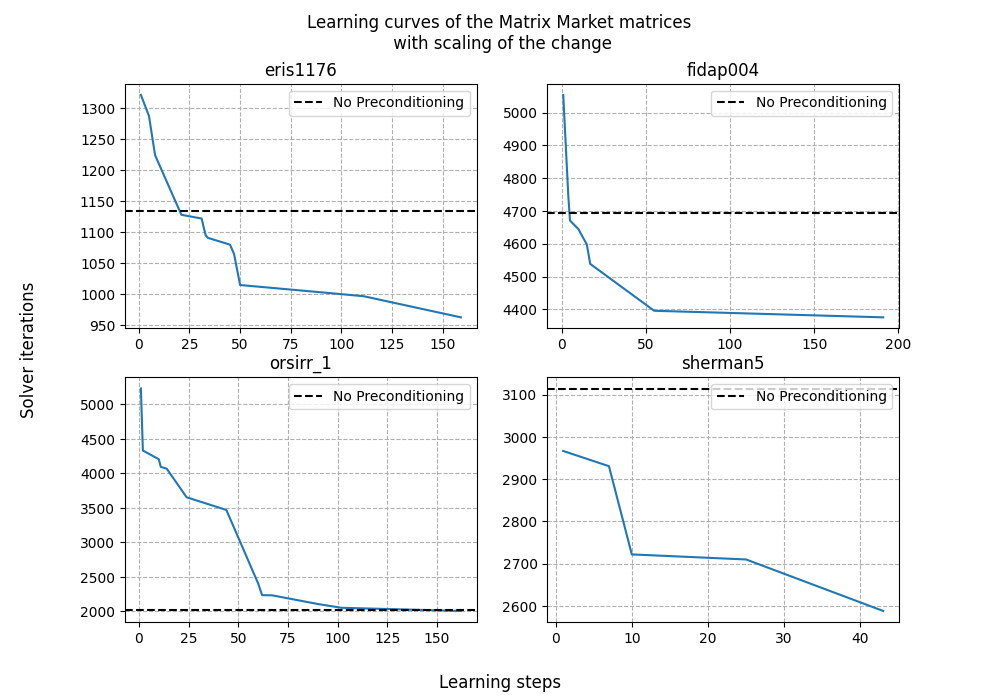
\includegraphics[width=0.8\textwidth]{plots/change_scale.png}
    \caption{Learning curves with scaling the change during learning for the four different test matrices. Where the blue line shows the solver iteration count, with a data point for each learning step the algorithm accepted a new preconditioner, and a dashed line indicating the unpreconditioned solver iteration count for corresponding matrix.}
    \label{fig: change of scale}
\end{figure}

\begin{table}[H]
    \center
    \begin{tabular}{|l|c|c|c|c|}
        \hline
        Matrix & Final & Compare v Non & \begin{tabular}{@{}l@{}}Learning\\ improvement\end{tabular} & \begin{tabular}{@{}l@{}}Number of \\ improvements\end{tabular}\\ \hline
        eris1176 & 963  & 171& 358 & 14 \\
        fidap004 & 4376  & 319& 678 & 8 \\
        orsirr\_1 & 2007  & 18& 3224 & 13 \\
        sherman5 & 2588  & 527& 379 & 5 \\\hline
    \end{tabular}
    \caption{Table of data from the learning of the preconditioner with scaling the change of the preconditioner with a row for each for the matrices and columns corresponds as table \ref{table: initial learn stat}.}
    \label{table: initial change stat}
\end{table}
